\documentclass[12pt]{article}

\usepackage{fullpage}
\usepackage{graphicx}
\usepackage{graphics}
\usepackage{mdwlist}
\usepackage{amsmath}
\usepackage{subcaption}
\usepackage{booktabs}
\usepackage{multicol}

% more space between table rows and columns
\renewcommand{\arraystretch}{1.15}

\setlength{\oddsidemargin}{0.0in}
\setlength{\evensidemargin}{0.0in}
\setlength{\textwidth}{6.5in}
\setlength{\headheight}{0.0in}
\setlength{\topmargin}{0.0in}
% \setlength{\textheight}{9.0in}
\setlength{\textheight}{9in}
\addtolength{\textheight}{-\topmargin}
\addtolength{\textheight}{-\headheight}
\addtolength{\textheight}{-\headsep}
\addtolength{\textheight}{-\footskip}

% bigger abstract margins
\let\oldabstract\abstract
\let\oldendabstract\endabstract
\makeatletter
\renewenvironment{abstract}
{\renewenvironment{quotation}%
               {\list{}{\addtolength{\leftmargin}{3em} % change this value to add or remove length to the the default
                        \listparindent 1.5em%
                        \itemindent    \listparindent%
                        \rightmargin   \leftmargin%
                        \parsep        \z@ \@plus\p@}%
                \item\relax}%
               {\endlist}%
\oldabstract}
{\oldendabstract}
\makeatother

% spacing in itemize environments
\usepackage{enumitem}
\setitemize{itemsep=1pt}

\begin{document}

\newcommand{\beq}{\begin{equation}}
\newcommand{\eeq}{\end{equation}}
\newcommand{\bit}{\begin{itemize*}}
\newcommand{\eit}{\end{itemize*}}
\newcommand{\goal}[1]{ {\noindent {$\Rightarrow$} \em {#1} } }
\newcommand{\hide}[1]{}
\newcommand{\comment}[1]{ {\footnotesize {#1} } }
\newtheorem{lemma}{Lemma}
\newtheorem{theorem}{Theorem}
\newtheorem{proof}{Proof}
\newtheorem{defn}{Definition}
\newtheorem{algo}{Algorithm}
\newtheorem{observation}{Observation}

\title{Leveraging network topology for better fake account detection in social networks\footnote{working title}}


\author{ {\em Björn Bebensee} \\
	    Dept. of Comp. Science and Eng.\\
	    Seoul National University\\
	    {\tt bebensee@snu.ac.kr}
	 \and
	 {\em Nagmat Nazarov} \\
	     Dept. of Comp. Science and Eng.\\
	     Seoul National University \\
	     {\tt nagmat@snu.ac.kr }
        }
\date{}

\maketitle
\begin{abstract}
    What is the Biggest Enemy of Social Media and social platforms?  
In this project, we develop {\em BOT detection methodology},
since animated social agents, or bots are increasingly becoming a huge problem on social media platforms.

\end{abstract}

\section{Introduction}
    \label{sec:intro}
    % {\em
% \bit
% \item
% what is the problem
% \item
% what are the applications
% \eit
% }
Today people all around the world use online social networks (OSNs) not only for personal connections but also for entertainment, to share opinions, to read news and inform themselves and to exchange knowledge and information. With their rise in popularity OSNs in the past decade however, they have become a target for abuse by malicious actors who are spamming the network, attempting to scam users, distribute malware, boost a legitimate user's popularity or increase the visibility of certain content. Furthermore with the 2016 United States presidential election the focus has been on social media rather than traditional media for the first time and the concern over widespread \emph{fake news} influencing public opinion as well as social bots pushing state-actor agendas has been growing~\cite{allcott2017social,grinberg2019fake} with some recent research focusing on identifying fake news using data mining methods~\cite{shu2017fake}.

Many OSNs spend a considerable amount of money and time in the form of manual labor on identifying and removing fake accounts. Our goal is to build on previous research and to improve the classification process for more effective and efficient identification of fake accounts. Unlike other approaches which focus only on basic profile features~\cite{cresci2015fame,malhotra2012studying} or temporal patterns in account activity~\cite{chavoshi2017temporal,ferraz2015rsc,gurajala2015fake}, our approach belongs to a category of graph-based approaches to fake account identification.  

Given the directed graph $G=(V,E)$ induced by the social network's structure as well as additional classification features $m_v$ for every $v \in V$, we want to identify all nodes $v \in V$ that are likely to correspond to fake accounts. We call this graph a social graph (figure \ref{fig:social_graph}). For social networks with bidirectional connections i.e. through friend requests an undirected graph may be used to describe the network structure. It is however vital for the classification task that the false-positive rate be kept low as suspensions of legitimate user accounts can degrade the experience enormously.


\begin{figure}
    \centering
    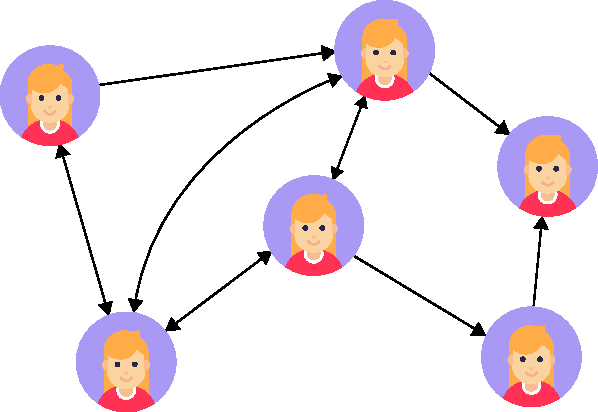
\includegraphics[width=0.4\textwidth]{FIG/social_graph}
    \caption{A social graph}
    \label{fig:social_graph}
\end{figure}


% INCLUDE CONTRIBUTIONS HERE LATER

%The contributions of this project are the following:
%\bit
%\item our proposed {\em someMETHOD} is novel, combining wavelets
%      with a spike-removal  preprocessing step
%\item it is effective, achieving 90\% classification accuracy
%\item it is scalable, being linear on the number of sound-clips $N$.
%\eit

In this paper we propose a novel approach to identification of fake accounts in OSNs by exploiting differences between the ego networks of legitimate users and fake accounts as well as weak links between communities of real users and communities of fake accounts. We first obtain a labelled dataset of legitimate and fake accounts on Twitter. As Twitter's developer policy limits the ways in which scraped user data may be published, these datasets typically contain a list of user IDs which we will then have to scrape to construct the social graph. We will explore this social graph and run experiments to find predictive features based on which we develop a novel approach. Finally, we evaluate our approach in experiments against other popular approaches for fake account detection in OSNs.

The rest of this paper is structured the following way: first we do a short survey of related work and their approaches (Section \ref{sec:survey}), based on the findings in these papers we will explore a dataset of Twitter users and fake accounts and their social graph, propose our own classification method, and evaluate our approach in experiments.

\section{Related Work}
    \label{sec:survey}
    In this section we will list papers that each member has read and reviewed as part of a first survey into the topic, along with a summary of their main ideas, how they can be of use for our own approach and possible shortcomings of the approach or important points not addressed by the paper.

%Table \ref{tab:symbols} gives a list of common symbols we used.
%\begin{table}[htb]
%\begin{center} 
%\begin{tabular}{|l | c | } \hline \hline 
%Symbol & Definition \\ \hline
%$N$ & number of sound-clips \\
%$D$ & average duration of a sound-clip \\
%$k$  & number of classes \\ \hline
%\end{tabular} 
%\end{center} 
%\caption{Symbols and definitions}
%\label{tab:symbols}
%\end{table} 

\subsection{Papers read by Björn Bebensee}

\subsubsection{Detecting Clusters of Fake Accounts in Online Social Networks}

\paragraph{Main idea:}
As opposed to previous literature which approaches the fake account classification problem on a per-account basis, Xiao, Freeman and Hwa~\cite{xiao2015detecting} suggest a different approach which uses an approach based on clustering instead. They suggest that as more efficient way of identifying a set of spam accounts made by a single spammer, one might classify entire clusters of users to be legitimate or fake instead of single user accounts. Furthermore their approach focuses on identifying and removing fake accounts before they can interact with legitimate users and spam the network so as to prevent damaging the experience of legitimate users. As they want to stop fake accounts as early as possible and only limited information becomes available during registration Xiao et al. focus on these few features which are available at registration time.

The authors divided their machine learning pipeline into three major parts: a cluster builder, a profile featurizer and an account scorer. The cluster builder takes a raw list of accounts and builds clusters of accounts where the clustering criteria can be simple (i.e. share a common feature) or more complex (like $k$-means). These clusters, along with the features needed for the profile featurizer, are then labelled as real or fake. If there are accounts of both groups in one cluster, it is labelled according to a threshold $x$. The featurizer extracts features from the set of accounts in one cluster to find a numerical representation (an \textit{embedding}) which can then be used by the account scorer to score the cluster. The authors test a number of models for the account scorer, specifically logistic regression, random forests and support vector machines. They find that for their use-case random forests perform best, with a recall slightly better than SVMs. Overall the model showed good performance in tests on in-sample data as well as a newer out-of-sample dataset. The authors have sinced deployed it in production at linked in and restricted more than 250,000 accounts.

\paragraph{Use for our project:}
This paper is closely related to the approach we want to take to classify accounts as genuine or as fake. Xiao et al. suggest classifying entire clusters of users rather than single users to leverage similarities between fake accounts. This technique could prove useful for our approach and can be used in combination with features from each user's social graph. It might be possible to cluster users based on graph features such as degree, number of triangles a node is part of and others.

\paragraph{Shortcomings:}

\subsubsection{Botnet detection using graph‐based feature clustering}

\paragraph{Main idea:}
In this paper Chowdhury et al.~\cite{chowdhury2017botnet} explore the use of graph-based features for clustering in computer networks to detect botnets. As much prior literature has focused on flow-based or rule-based detection, the authors suggest using clustering to first identify clusters of suspicious nodes. The authors are using a self-organizing map (SOM) for dimensionality reduction and clustering by assigning each node to a different cluster according to the output of the SOM. The features used for clustering are node in-degree, out-degree, in-degree weight (i.e. how many packets are received), out-degree weight (i.e. number of outgoing packets), clustering coefficient, node betweenness, and eigenvector centrality. Finally they are classifying nodes in each cluster (except the largest as it is unlikely to contain bots) starting from the smallest cluster using their own bot-search algorithm which only requires examination of few nodes for classification.
Chowdhury et al. show that their approach performs better than SVM classification on the CTU-13 dataset (a dataset of botnet traffic) using the same graph features.

\paragraph{Use for our project:}
Although the approach presented in the paper operates on an entirely different set of data, it is very similar to our goal in its nature. The authors want to identify a set of bad actors in a network given interactions between devices and given the network structure. As we are attempting to classify users in a social network according to the structure and topology of the social graph, we aim to use a set of graph-based features, similar to the features used in the paper, to cluster groups of users which we may subsequently classify jointly.

\paragraph{Shortcomings:}
Calculating all given graph features for all nodes in the graph will not scale very well. For the CTU-13 dataset used by the authors the computation took 30 hours on a supercomputer cluster. This is not an acceptable amount of processing power and time to detect social bots in social networks in (near) real-time in order to prevent interactions with real users. However, as the CTU-13 dataset contains much data and information that is not contained or necessary for an application on social graphs, some of the ideas from these paper may still viable in our use-case. Further experimentation is required.

\subsubsection{Aiding the detection of fake accounts in large scale social online services}

\paragraph{Main idea:}
Cao, Sirivianos, Yang and Pregueiro~\cite{cao2012aiding} build on previous work in \emph{sybil detection} that aims to use random walks to identify fake accounts (\emph{sybils}) based on key observations made on the structure of social graphs. Specifically a main assumption in these fake account detection schemes is that the connectivity between real users and fake accounts is limited and lower than the number of inter-user and inter-bot connections. In this work Cao et al. propose a new algorithm called SybilRank which, unlike previous work in the field, does not aim to make a binary classification of each user account but instead focuses on creating a ranking which allows for a measure of confidence in classifications as well as further challenges like \emph{captchas} for suspicious accounts. The key idea behind this algorithm is that in a social network an early-terminated random walk starting from a real user account has a higher probability of landing at another real-user than at a fake account. Early termination is necessary for these random walks as the probability of landing at any node converges to a uniform distribution for random walks of sufficient length. The authors can thus use the degree-normalized landing probability of early-terminated random walks to rank nodes and leverage the fact that connections between real users and fake accounts are limited. They further propose a more effecient way of calculating the landing probability of random walks using power iteration.


\paragraph{Use for our project:}
Use for our project: Cao et al. show that it is possible to leverage the topology of the social graph, specifically the weak links between fake accounts and real users, to identify these fake accounts. As we plan to use binary classification for this task, it could prove helpful to include the degree-normalized landing probability for random walks as an additional graph feature either in the machine learning algorithm or for clustering of similar nodes, given that it can be computed efficiently enough which may not be the case for large-scale social networks.

\paragraph{Shortcomings:}
The authors suggest running the SybilRank algorithm periodically, i.e. once every month, which would give fake accounts a window of time that is big enough to interact with and impact real users' experience on the social network unlike the approach introduced by Xiao et al.~\cite{xiao2015detecting}.

\subsection{Papers read by Nagmat Nazarov}



\subsubsection{Towards a language independent Twitter bot detector}

\paragraph{Main idea:}
The authors present a language independent approach to classify each single tweet to be either auto generated(AGT) or human-generated(HGT). Jonas Lundberg, Jonas Nordqvist and Mikko Laitinen ~\cite{lundberg2019towards} The AGT classifier consists of 10 tweet properties. They are a) \textit{isreply}, b) \textit{isRetweet}, C) \textit{accountReputation} - number of followers divided by number of friends and followers, d) \textit{hashtagdensity},\textit{urldensity}, \textit{mentiondensity} e) \textit{statusperday} f) \textit{favoritesperday} and g) \textit{devicetype}. 
On this paper rather than evaluating all applicable machine learning algorithms(like on the other papers) they prefered tree-based models since they outperform well. The results are generated by J48 and RandomForest tree-based models.   
\paragraph{Use for our project:}
We may use RandomForest tree-based algorithm for detection of bot accounts on online social platforms, since it performed the best training results(error rate 3.73\text{\%}) on this paper.  
\paragraph{Shortcomings:}





\subsubsection{A network topology approach to bot classification}

\paragraph{Main idea:}
The authors are proposing a Network Topology approach to Bot classification problem on online social media platforms. Nowadays automated social agents, or bots are increasingly becoming problematic on social media platforms. Laurewz A Cornelissen, ~\cite{cornelissen2018network} Richard Barnett, Petrus Schoonwinkel,Brent Eichstadt and Hluma Magodla are proposing that the social network topology of a user would be sufficient to determine whether the user is a automated agent or a human. Using an unsupervised machine learning approach, a detection accuracy rate of 70\text{\%} is reached.
A new specialised approach, using ego-centred network topology as feature vectors for unsupervised machine learning was proposed on this paper. 
\cite{cornelissen2018network}

\paragraph{Use for our project:}
The authors suggest to use centrality graph measure, for example celebrities have high indegree and low outdegree. For instance, celebrities on Twitter tend to have more people following them than they follow themselves. The authors also propose that the bots must have high outdegree but very low indegree, since most people will not follow back. We can use this proposal to distinguish the bots with non bots. ~\cite{cornelissen2018network} 
\paragraph{Shortcomings:}




\subsubsection{Bot Classification for Real-Life Highly Class-Imbalanced Dataset}

\paragraph{Main idea:}
Generally the researches on bot detection is based on particular botnet characteristics, but in this paper the authors develop three generic features to detect different types of bots regardless of their botnet characteristics. Sarah Harun, Tanveer Hossain Bhuiyan, Song Zhang, Hugh Medal and Linkan Bian~\cite{harun2017bot} suggest five classification models based on those features to classify bots from a large, real-life class-imbalanced network dataset. The authors think that the generalized bot detection methods perform better than the botnet specific methods. 
The bot detection methodology is at first filtering out the unnecessary data and then apply feature extractor to the rest of data. Filtering : The authors filter the IPs which never act as a source and remove IPs which perform only single communication with other IP. After that the bots are extracted based on assumptions of bot behavior according to 1) Falling rate of communication frequency, 2) media communication frequency and 3) source bytes per packet for highest communication frequency.  To develop classification models using these features. The supervised learning algorithms like Quadratic discriminant analysis, Gaussian Naïve Bayes, Support Vector Machine, K Nearest neighbor and Random Forest are used. 
\paragraph{Use for our project:}
The classification results are analyzed according to 6 scenarios , as a result Quadratic discriminant analysis and Gaussian Naïve Bayes perform much better than others. These two supervised learning algorithms are closely related to the approach we want to take to classify accounts as bots or nonbot.  
\paragraph{Shortcomings:}
The biggest shortcoming of this paper is that it ignores the passive or less active bots from the  beginning. I think less active bots can be initiated instead of single very active bot. Another shortcoming is that the paper does not take into account passive bots from the beginning, which may harm the real users by the time. 

% Progress report

\section{Proposed Method}
    \label{sec:proposed}
    In this section we will briefly describe and analyze the dataset used in this work. In section~\ref{sec:approach} describe our novel approach and how we train the classification model in detail.

% BIG TWITTER HAIRBALL GRAPH
\begin{figure}[t!]
    \centering
    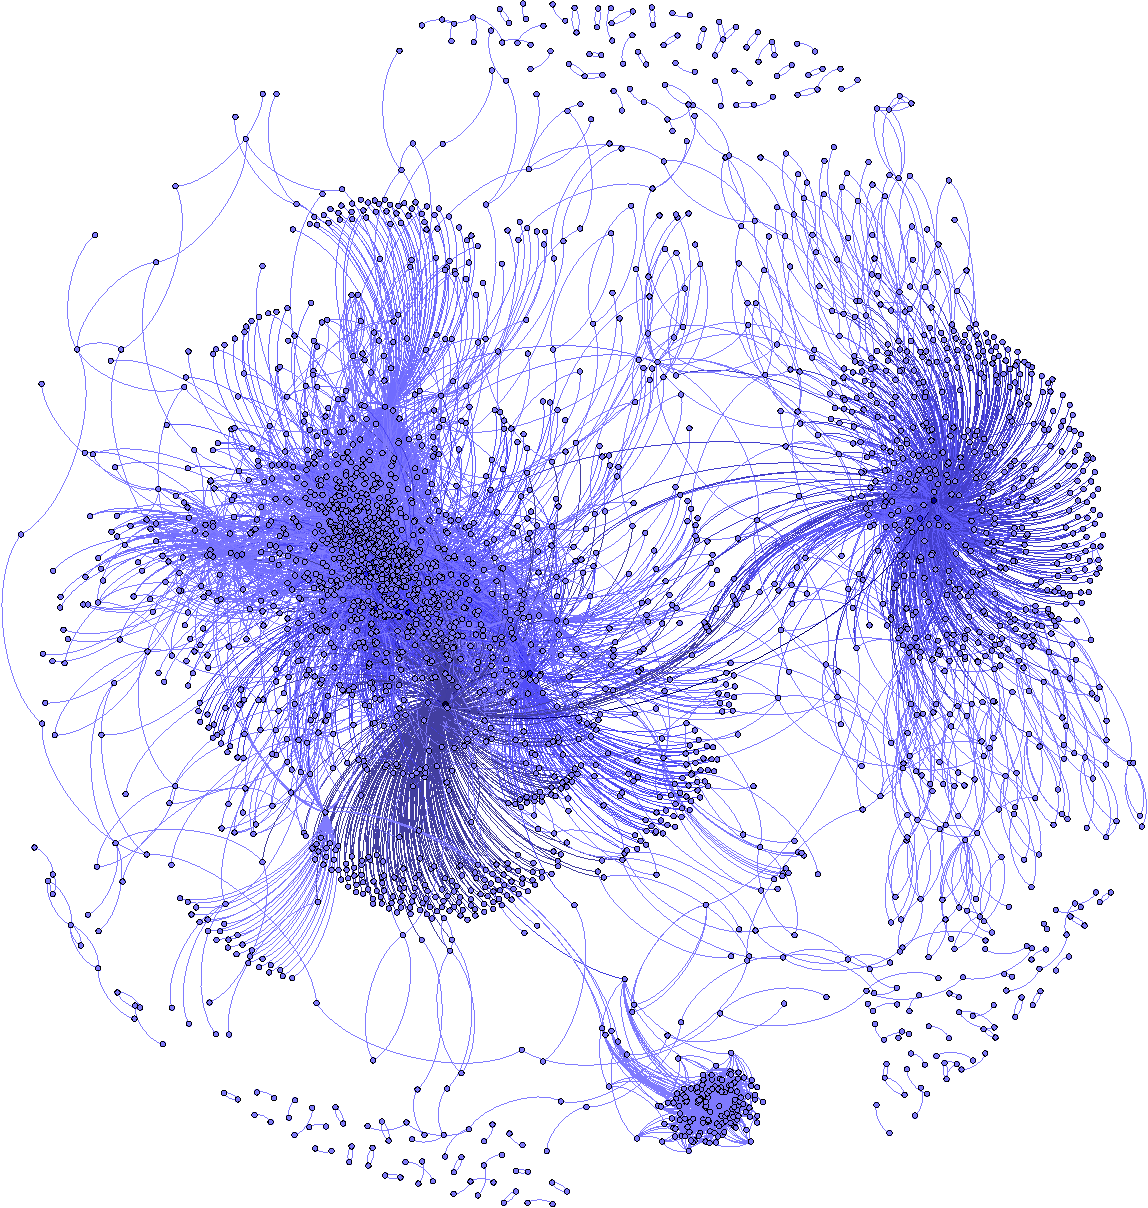
\includegraphics[width=0.5\textwidth]{FIG/graph-crop.pdf}
    \caption{A visualization of the dataset. Each vertex corresponds to a Twitter user and each edge corresponds to a ``following" relationship between two users. A darker node has a higher degree. We can see many disconnected components.}
    \label{fig:twitter}
\end{figure}

\subsection{Dataset}
For analysis, training and testing we use the labelled data collected in the \textsc{Cresci-2018} dataset~\cite{cresci2018fake}. The dataset contains 25,987 user accounts, each of which is assigned a binary label $l \in \{\text{human},\text{bot}\}$ and is the biggest one of its kind that we are aware of. Due to Twitter's developer policy\footnote{https://developer.twitter.com/en/developer-terms/agreement-and-policy.html} which restricts the ways in which user data collected using the Twitter API may be shared, it is difficult to find sizable high-quality datasets. As the rules allow for profile data to be shared online only under specific circumstances and with imposed restrictions, these datasets of fake accounts are typically shared as a set of (user\_id, label) pairs. The associated accounts can then be retrieved again using the Twitter API at a later time. However, as many of the labelled accounts are bots might have been deleted or changed to a ``protected" status which hides most of the profile information from the public. In our case, even though the dataset is relatively recent, only 13,091 of the originally 25,987 labelled accounts were still available (a reduction of about 49.6\%). Of these 6,082 accounts are labelled to be human and 7,009 accounts are labelled as bots (see table~\ref{tab:dataset}).

\begin{table}[t]
\centering
\begin{tabular}{@{}lllllll@{}}
\toprule
       &  & \multicolumn{2}{l}{Ours} &  & \multicolumn{2}{l}{\textsc{Cresci-2018}} \\ \midrule
Humans &  & 6,082       & 46.46\%     &  & 7,479          & 28.78\%         \\
Bots   &  & 7,009       & 54.54\%     &  & 18,508         & 71.22\%         \\ \midrule
\textbf{Total}  &  & \textbf{13,091}      &        &  & \textbf{25,987}         &            \\ \bottomrule
\end{tabular}
\caption{Dataset distribution after retrieving available user profiles using the Twitter API}
\label{tab:dataset}
\end{table}

In addition to the labelled user accounts we have collected all profiles of users followed by or following a user in the dataset. As the Twitter API limits us to a maximum of the first 5,000 users when retrieving these lists we only get those first 5,000 users for users following or followed by more than 5,000 accounts. Including these user profiles we have a total of 4.6 million user profiles. For each user we have the following attributes:

\begin{multicols}{2}
\begin{itemize}
    \item user ID
    \item label
    \item username
    \item screen name
    \item number of “followers” (in-degree)
    \item number of “following” (out-degree)
    \item location
    \item profile URL
    \item profile description
    \item number of times the user is listed
    \item number of favourites
    \item number of status
    \item date created
    \item default profile (boolean)
    \item default profile image (boolean)
    \item list of users followed (up to 5000)
    \item list of followers (up to 5000)
\end{itemize}
\end{multicols}

From this data we can recreate the social graph with distance $d\leq2$ from the users in the \textsc{Cresci-2018} dataset as we have the number of followers and users followed for all users of distance $d=1$ which allows us to simply create ``dummy" nodes without any other attributes in the graph. Unfortunately scraping user profiles of distance $d\geq3$ from the original dataset does not seem feasible for us as this would seem to include a large part of all Twitter accounts and given the Twitter API restrictions might take months. For reference the $90^{th}$-percentile effective diameter of Twitter in 2010 was 4.8~\cite{kwak2010twitter}. A visualization of the graph of all labelled nodes can be seen in figure~\ref{fig:twitter}.

Given this data we perform some basic analysis. When plotting the in-degree-count and out-degree-count graphs we can easily see that bot users tend to have a lower in-degree (less followers) and also a lower out-degree (following less users) than human users. It is worth noting that while the bot accounts seem to mostly follow a power-law, the out-degree distribution for human accounts does not follow a power-law and many nodes in the dataset appear to have a surprisingly high out-degree that may not be perfectly representative of the general user population on Twitter. Further analysis shows that the clustering coefficient of both human and bot accounts appears to be rather low overall which can be explained to the lack of edges and paths that are not included due to the limitations of our crawl of the Twitter network (see figure~\ref{fig:centrality_clustering}). However, we find that the clustering coefficient of human accounts is still slightly higher than that of bot accounts. Regarding the eigenvector centrality we find that human accounts have a slightly higher value too (see also figure~\ref{fig:centrality_clustering}). We believe that these findings may be stronger in a more comprehensive dataset and warrants further investigation in future work.

% GENERAL DEGREE DISTRIBUTION
\begin{figure}[t!]
    \centering
    \begin{subfigure}[t]{0.5\textwidth}
        \centering
        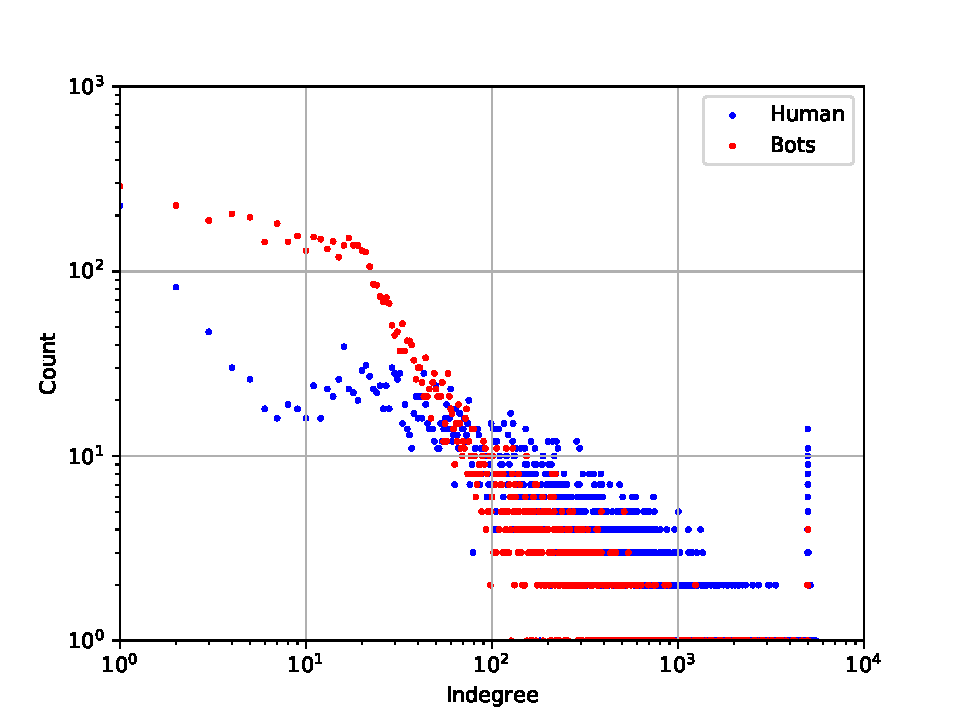
\includegraphics[width=\textwidth]{FIG/indegrees.pdf}
        \caption{In-degree-count graph}
    \end{subfigure}%
    ~
    \begin{subfigure}[t]{0.5\textwidth}
        \centering
        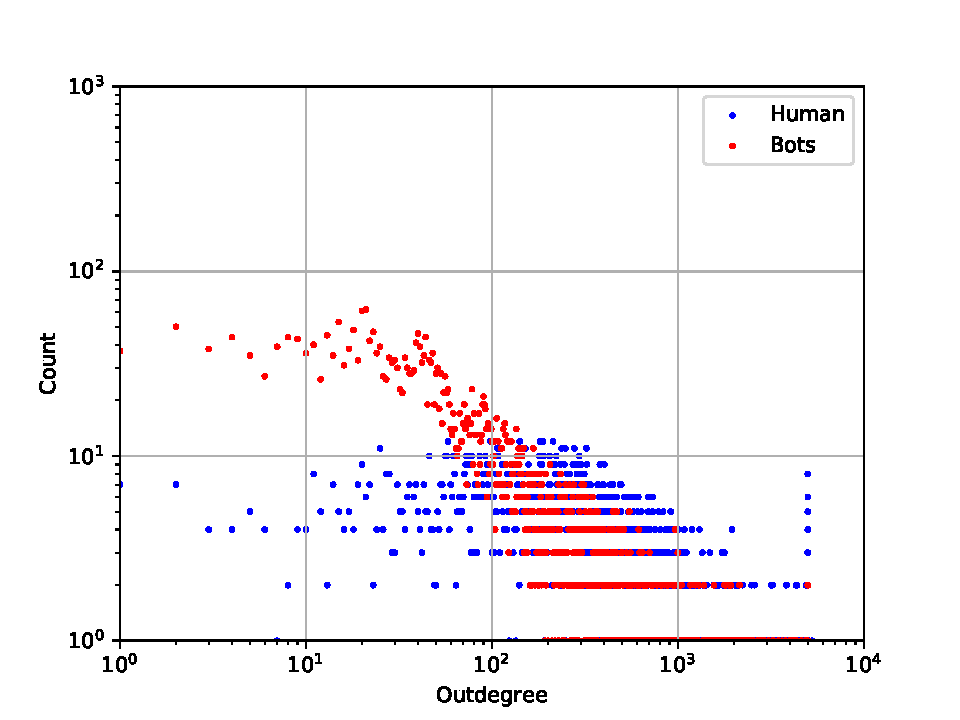
\includegraphics[width=\textwidth]{FIG/outdegrees.pdf}
        \caption{Out-degree-count graph}
    \end{subfigure}
    \caption{Degree-count graphs for human and bot accounts}
    \label{fig:degrees}
\end{figure}

% CENTRALITY AND CLUSTERING COEFFICIENT
\begin{figure}[t!]
    \centering
    \begin{subfigure}[t]{0.5\textwidth}
        \centering
        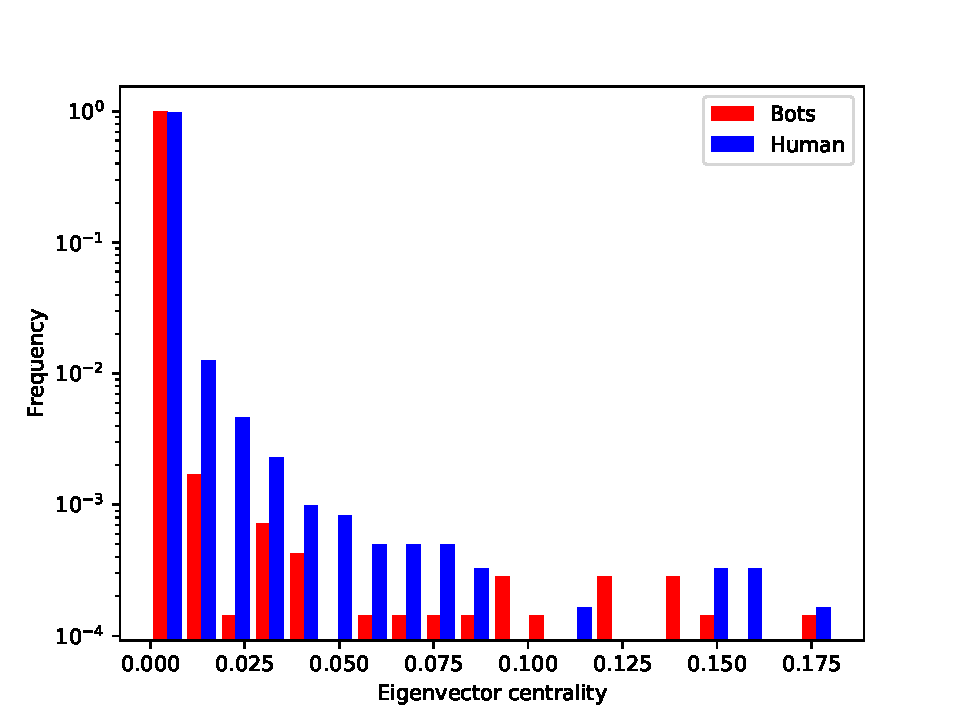
\includegraphics[width=\textwidth]{FIG/centrality.pdf}
        \caption{Eigenvector centrality-frequency graph}
    \end{subfigure}%
    ~
    \begin{subfigure}[t]{0.5\textwidth}
        \centering
        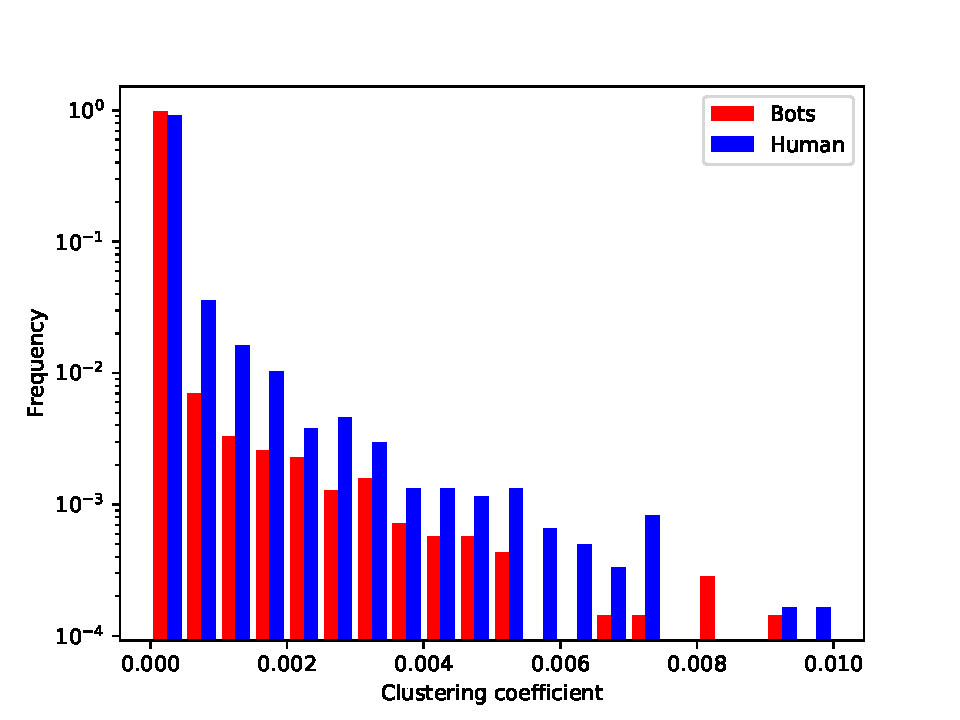
\includegraphics[width=\textwidth]{FIG/coefficient.pdf}
        \caption{Clustering coefficient-frequency graph}
    \end{subfigure}
    \caption{We compare the eigenvector centrality and clustering coefficient distributions among human and bot accounts.}
    \label{fig:centrality_clustering}
\end{figure}


\subsection{Neighborhood-based classification}
\label{sec:approach}

We introduce a novel graph topology and neighborhood-based approach to bot detection. Human and bot accounts typically differ in the way they use Twitter and as a result their structure in the social graph, or their ego graph, is typically different. Instead of classifying a node in the graph just by its immediate features (such as follower count, number of tweets, default profile image etc.) we propose to utilize the graph structure and the features of neighboring nodes in bot classification. We introduce an additional set of features computed as an aggregate over the entire set of predecessors and/or successors. 

% REPUTATION
\begin{figure}[t!]
    \centering
    \begin{subfigure}[t]{0.5\textwidth}
        \centering
        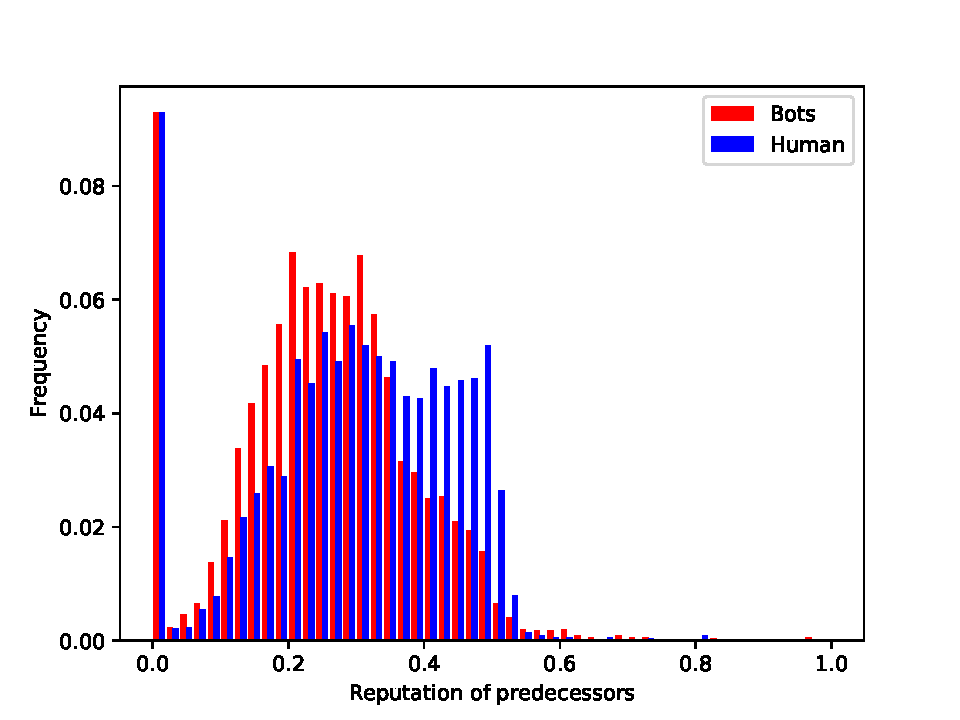
\includegraphics[width=\textwidth]{FIG/reputation_pre.pdf}
        \caption{Aggregated reputation of predecessors}
    \end{subfigure}%
    ~ 
    \begin{subfigure}[t]{0.5\textwidth}
        \centering
        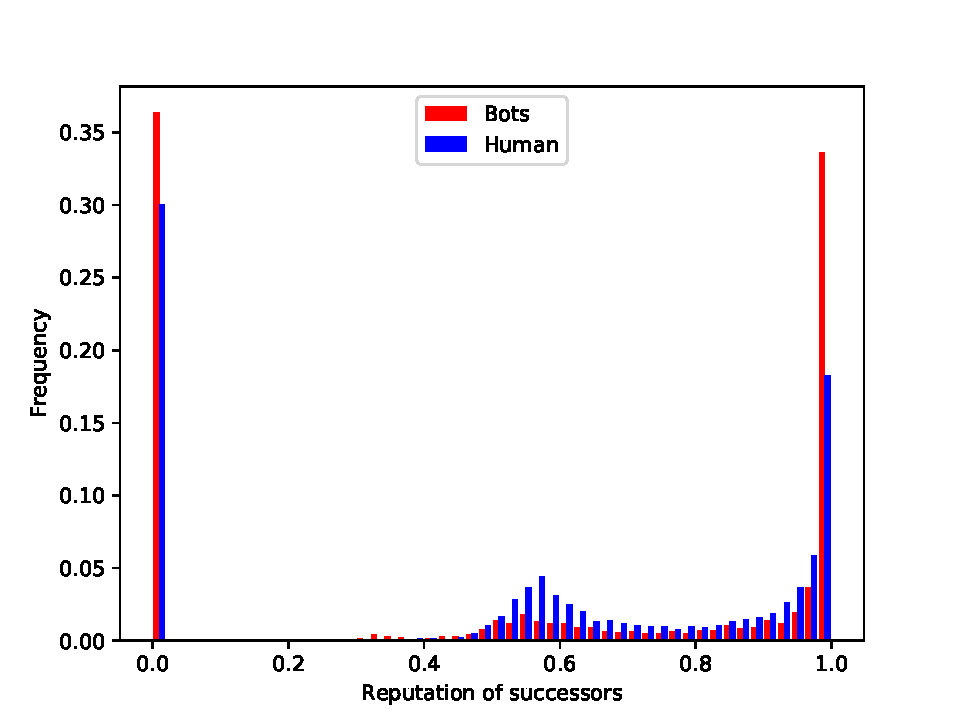
\includegraphics[width=\textwidth]{FIG/reputation_succ.pdf}
        \caption{Aggregated reputation of successors}
    \end{subfigure}
    \caption{We compare the aggregated reputation of users following (predecessors) or followed by (successors) a given user over all human and bot accounts.}
    \label{fig:reputation}
\end{figure}

We will first compute such aggregate features for the dataset using the social graph. In addition to the features scraped using the Twitter API, we computed and evaluated the following features during our analysis. An aggregate of a  feature for a user's neighborhood (a \emph{neighborhood feature}) can be computed by taking the median value across all predecessors or successors (see figure~\ref{fig:reputation}). An aggregate of this measure can be computed across all predecessors/successors by taking the median (see figure~\ref{fig:reputation}).

% DEGREE PREDECESSORS
\begin{figure}[t!]
    \centering
    \begin{subfigure}[t]{0.5\textwidth}
        \centering
        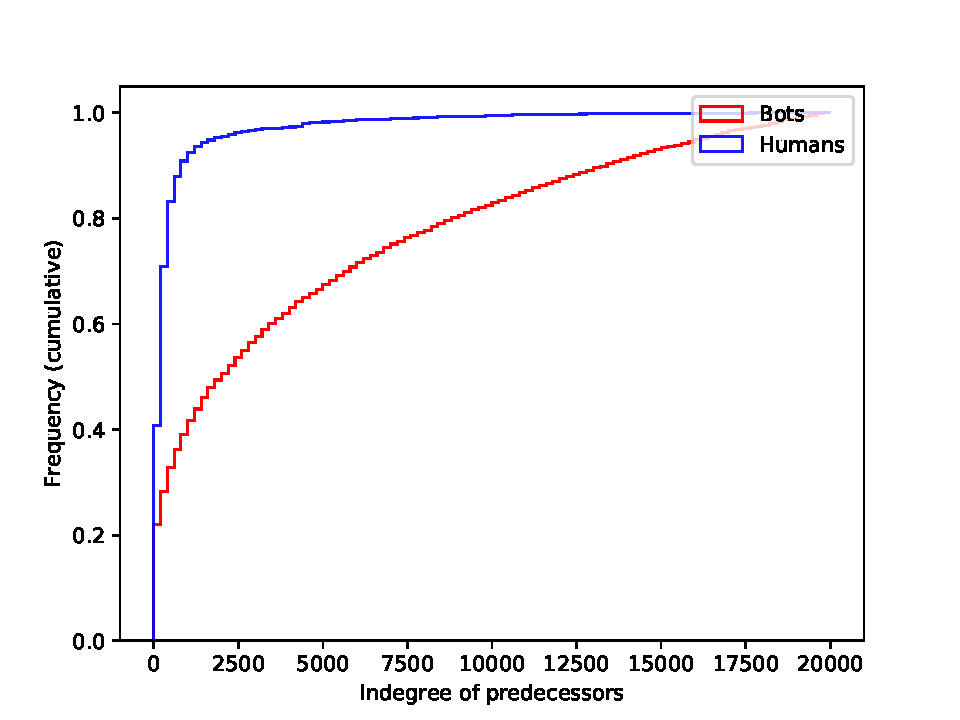
\includegraphics[width=\textwidth]{FIG/indegree_pre.pdf}
        \caption{in-degree}
    \end{subfigure}%
    ~ 
    \begin{subfigure}[t]{0.5\textwidth}
        \centering
        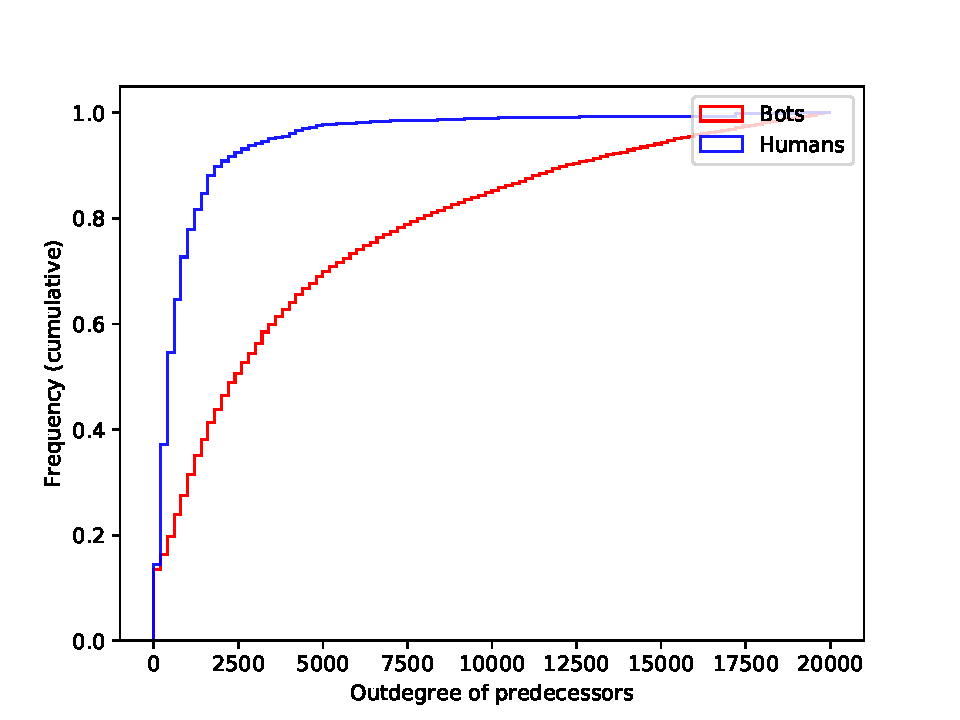
\includegraphics[width=\textwidth]{FIG/outdegree_pre.pdf}
        \caption{out-degree}
    \end{subfigure}
    \caption{Cumulative aggregated degree distribution of predecessor nodes, i.e. median degree of users following by a given user over all bot and human accounts.}
    \label{fig:cum_degrees_predecessors}
\end{figure}

% DEGREE SUCCESSORS
\begin{figure}[t!]
    \centering
    \begin{subfigure}[t]{0.5\textwidth}
        \centering
        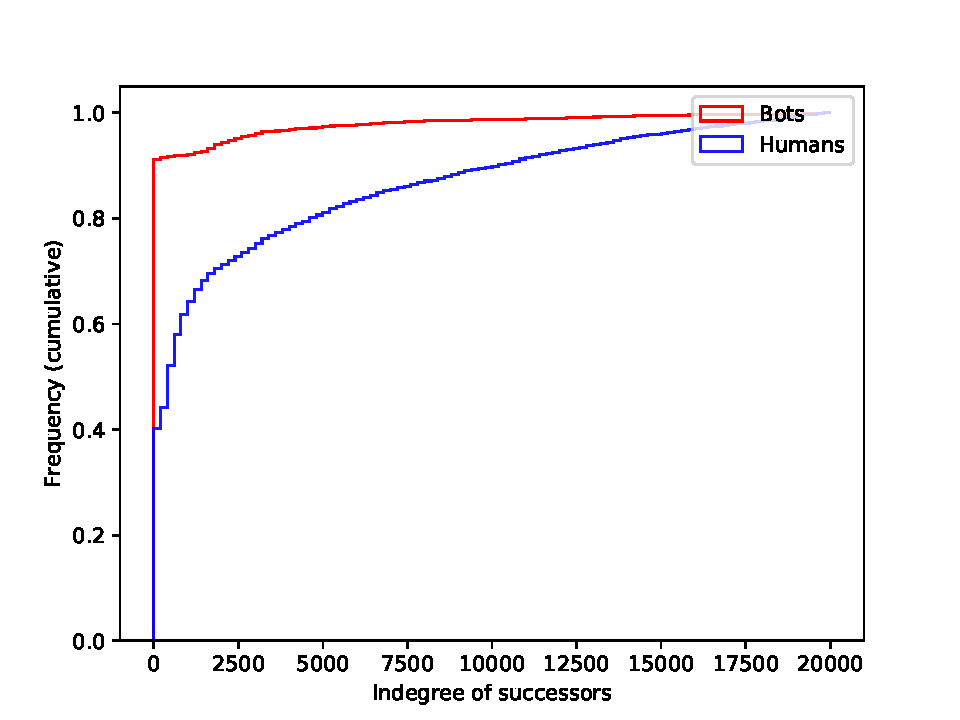
\includegraphics[width=\textwidth]{FIG/indegree_succ.pdf}
        \caption{in-degree}
    \end{subfigure}%
    ~ 
    \begin{subfigure}[t]{0.5\textwidth}
        \centering
        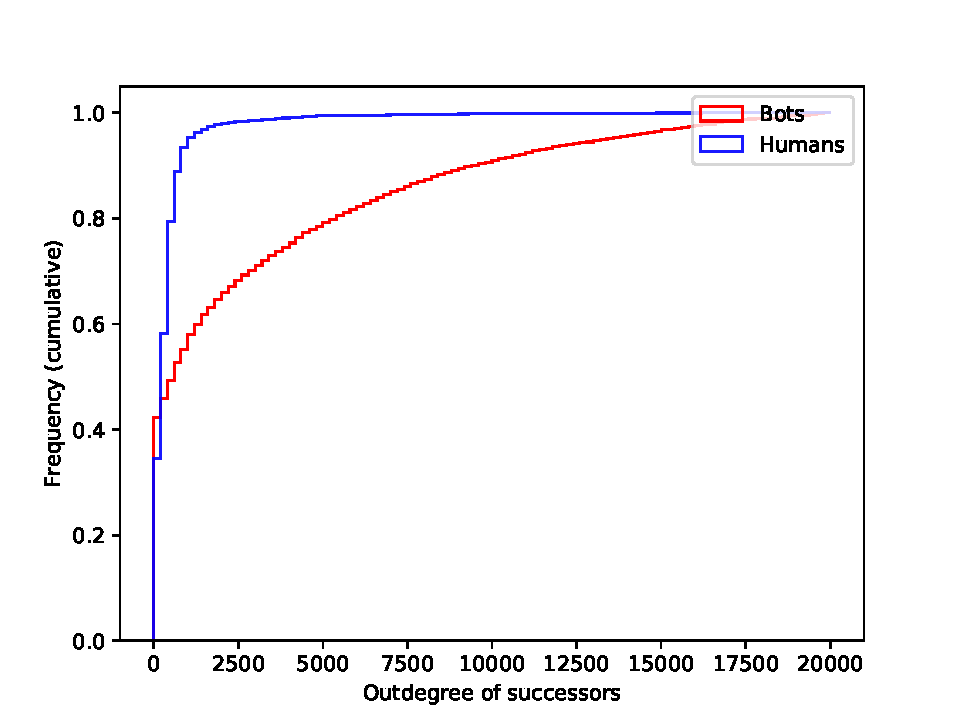
\includegraphics[width=\textwidth]{FIG/outdegree_succ.pdf}
        \caption{out-degree}
    \end{subfigure}
    \caption{Cumulative aggregated degree distribution of successors nodes, i.e. median degree of users followed by a given user over all bot and human accounts.}
    \label{fig:cum_degrees_successors}
\end{figure}

\paragraph{Reputation.} A user's reputation is often measured as the following/follower ratio. We define the reputation $r$ of a user $u$ by
\begin{align*}
    r_u = \frac{ |u_\text{followers}| }{ |u_\text{followers}| + |u_\text{following}|}.
\end{align*}

\paragraph{Median indegree.} We compute median indegree of successors and the median indegree of predecessors. Intuitively, we believe humans tend to follow more high-indegree users (i.e.) news sites, celebrities, while being followed by other low-indegree users.

\paragraph{Median outdegree.} We compute median outdegree of successors and the median outdegree of predecessors. The intuition is that bots may be more likely to be followed by bots or users that follow a large amount of people.

\paragraph{Median reputation.} The above measure of reputation, that is $r_u = \frac{ |u_\text{followers}| }{ |u_\text{followers}| + |u_\text{following}|}$, aggregated for predecessors and successors in the social graph each. Intuitively, real accounts 

\paragraph{Median status count.} Median of status updates for predecessors and successors in the social graph.

\paragraph{Median favourites count.} Median number of favourites or likes by a user's predecessors and successors.

\paragraph{Median listed count.} Median number of times a user's predecessors and successors appear in other users lists on Twitter.

\paragraph{Median account age.} The median account age of predecessors and successors in the social graph. Intuitively, older accounts tend to be more likely to be real users whereas recently created accounts may be bot accounts.

\paragraph{Number of egograph edges.} The total number of edges in a user's egograph. Used to measure how connected the egograph is.

\paragraph{Number of egograph nodes.} The total number of nodes in a user's egograph. Used to measure how connected a user is in the social graph.

\paragraph{Density.} The density of a user's egograph. A graph's density describes the number of edges in relation to the number of nodes. A complete graph has density 1 while a graph with an empty set of edges has density 0. For $n$ nodes and $m$ edges, it is computed as
\begin{align*}
    d_G = \frac{m}{n(n-1)}.
\end{align*}

\paragraph{Reciprocity.} We measure reciprocity in each user's egograph by computing the ratio of edges that are reciprocated (i.e. that point in both directions) to the total number of edges in the egograph. That is
\begin{align*}
   \mathrm{rec}_G = \frac{|\{(u,v) \ | \ (u,v) \in E \wedge (v,u) \in E \}|}{|\{ (u,v) \ | \ (u,v) \in E \}|}
\end{align*}

\paragraph{Assortativity.} A graph's assortativity measures the similarity of nodes in a graph given a certain attribute. In this case we choose to use ( indegree assortativity (i.e. follower assortativity) to describe how similar a user's egograph is in terms of indegrees.


\bigskip

We find that overall successors appear to have a higher reputation than predecessors. This observation makes sense as many users follow high-degree, high-reputation nodes such as news sources, which in turn are not likely to be following them back. We can also make the observation that human nodes tend to have more reputable predecessors. Additionally, the distribution of reputation of successors is extremely skewed to both extremes for bots which indicates most of them they either follow very reputable nodes or nodes with very low reputation. While the distribution is also extreme for humans, it is not skewed quite as strongly and has many more nodes with a reputation $0.1 < r < 0.9$.

When looking at the cumulative degree distribution among predecessors (figure~\ref{fig:cum_degrees_predecessors}) and successors (figure~\ref{fig:cum_degrees_successors}) we find that many bot accounts in the dataset have predecessors with very high in-degree and out-degree whereas most genuine accounts seem to have lower predecessor degree distributions. For successors however, human accounts tend to have successors with a higher in-degree and lower out-degree, which is in line with our observations regarding the reputation and again indicating that human users tend to follow more accounts with many followers such as news accounts or celebrities. 

%\noindent
%\textit{Logistic regression.} Given a set of $m$ trainings samples $S = \{ (x^{(i)}, y^{(i)}) \}_{i=1}^m$ where $x^{(i)}$ responds to the input features and $y^{(i)}$ in $\{ 0,1 \}$ to the labels, we can model logistic regression as
%$$
%p(y=1|x,\theta) = \frac{1}{1+\text{exp}(-\theta^T x)}
%$$
%with model parameters $\theta$.


\section{Experiments}
    \label{sec:evaluation}
    In this section we describe our model and compare it to a number of different baseline models. We implement our model as well as the baselines in Python 3.7 using NumPy, Pandas, Scikit-learn and PyTorch. We split the training data into training and test datasets randomly while ensuring that the distributions of human/bot labels in both datasets represent the overall distribution accurately.

\begin{figure}
    \centering
    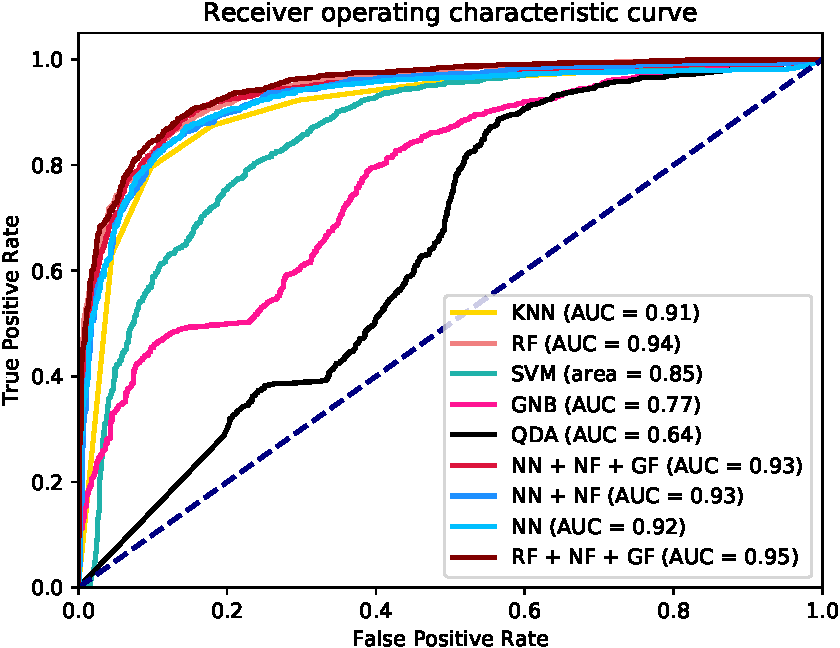
\includegraphics[width=0.65\textwidth]{FIG/roc-crop.pdf}
    \caption{ROC curve for our models and the baseline models}
    \label{fig:roc}
\end{figure}

We evaluate the model against Gaussian Naïve Bayes (GNB), Quadratic Discriminant Analysis (QDA), a Support Vector Machine (SVM), a $k$-Nearest Neighbors (KNN), a Random Forest (RF) and a neural network (NN) model. For these baseline models we use the following features:
\begin{align*}
    X_{base} = \{ & \texttt{default\_profile}, \texttt{profile\_image}, \texttt{favourites\_count}, \\
    & \texttt{followers}, \texttt{following}, \texttt{listed\_count}, \texttt{statuses\_count}, \\
    & \texttt{account\_age}, \texttt{reputation} \}
\end{align*}


After evaluating linear, polynomial and RBF kernels for the SVM model, we found the model to perform best with the RBF kernel. The RF model is trained using 100 trees, and splits are performed according to the Gini coefficient. GNB and QDA models are trained using the standard settings in Scikit-learn. 

The neural network classifier is a fully-connected feedforward neural network. After much experimentation we chose to use 3 hidden layers with $(500, 200, 200)$ neurons respectively, using batch normalization and dropout with $p=0.5$. The model is trained using Adam and a learning rate of $\eta = 0.001$ for 500 epochs. We find that the model achieves better performance and generalizes better when we remove outliers that deviate from the mean by more than three standard deviations from the training dataset.

We experimented with different sets of features and found a set of neighborhood features (NF) and graph features (GF) described in section \ref{sec:approach} that performs best along with the baseline features. We also found that removing some of the original features along with adding the  NF and GF improved the performance of our classification model. The final set of features used in our classifier are:
\begin{alignat*}{2}
    & X_{NF} = \{ && \texttt{favourites\_count}, \texttt{statuses\_count}, \texttt{outdegree\_predecessors}, \\
    & && \texttt{favorites\_predecessors}, \texttt{status\_predecessors}, \\
    & && \texttt{age\_predecessors}, \texttt{account\_age}, \texttt{following}, \texttt{followers} \} \\
    \\
    & X_{GF} = && \{ \texttt{ego\_density}, \texttt{ego\_reciprocity} \}
\end{alignat*}

\begin{table}[t]
\centering
\setlength{\tabcolsep}{12pt}
\begin{tabular}{@{}lccccc@{}}
\toprule
\textbf{Model} & \textbf{Accuracy} & \textbf{TPR} & \textbf{FPR} & \textbf{$\boldsymbol{F_1}$ score} & \textbf{AUC} \\ \midrule
GNB             & 0.6399 & \textbf{0.9622} & 0.7313 & 0.741  & 0.7652 \\
QDA             & 0.6751 & 0.8937 & 0.5768 & 0.7465 & 0.6405 \\
SVM             & 0.7797 & 0.7746 & 0.2145 & 0.7901 & 0.7801 \\
KNN             & 0.8496 & 0.8752 & 0.18   & 0.8617 & 0.9074 \\
RF              & 0.8675 & 0.8745 & 0.1405 & 0.876  & 0.9426 \\
NN              & 0.8648 & 0.8673 & 0.138  & 0.8729 & 0.9154 \\ \midrule
NN + NF (ours)  & 0.8702 & 0.8623 & \textbf{0.1208} & 0.8767 & 0.928 \\
NN + NF + GF (ours) & 0.8751 & 0.8894 & 0.1413 & 0.8841 & 0.9367 \\
RF + NF + GF (ours) & \textbf{0.8774} & 0.888 & 0.1348 & \textbf{0.8858} & \textbf{0.9468} \\
\bottomrule
\end{tabular}
\caption{Results on the \textsc{Cresci-2018} dataset for various baseline models (top) and our model using neighborhood features (bottom).}
\label{tab:results}
\end{table}

\noindent We denote the number of correctly positively classified samples as TPR (true-positive rate) whereas FPR is the number of falsely positively classified samples (false-positive rate). The models are evaluated in terms of:
\begin{itemize}
    \item[1.] Accuracy
    \item[2.] TPR
    \item[3.] FPR
    \item[4.] $F_1$ score
    \item[5.] area under the ROC curve (AUC)
\end{itemize}

Our model outperforms the baseline models on the \textsc{Cresci-2018} dataset (table~\ref{tab:results}). We notice that both the GNB and QDA model are not very good at identifying bot accounts on this dataset accurately and have a very high false positive rate. The SVM model is slightly better and achieves an $F_1$ score of 0.79. Interestingly, KNN is surprisingly effective on this dataset and only slightly less effective than the RF and NN models. Both RF and NN turn out to be very effective and achieve the highest scores. Due to this, we chose to focus only on the RF and NN models for our proposed extensions and sets of features. By using the proposed NF we see an overall improvement both for the RF and NN models.

It is interesting to note that only a set of certain, very few features is sufficient to effectively separate bots and humans in multi-dimensional space. We find that the number of a user's favourites, followers and statuses actually suffice to identify very clear differences in the distribution of human and bot accounts (figure \ref{fig:3dvis}). Indeed, a RF classifier is able to achieve an $F_1$ score of 0.8738 and AUC of 0.8659 using only those three features and actually performs better than all of the baseline models which were trained on all features retrieved using the Twitter API.

\begin{figure}[t]
    \centering
    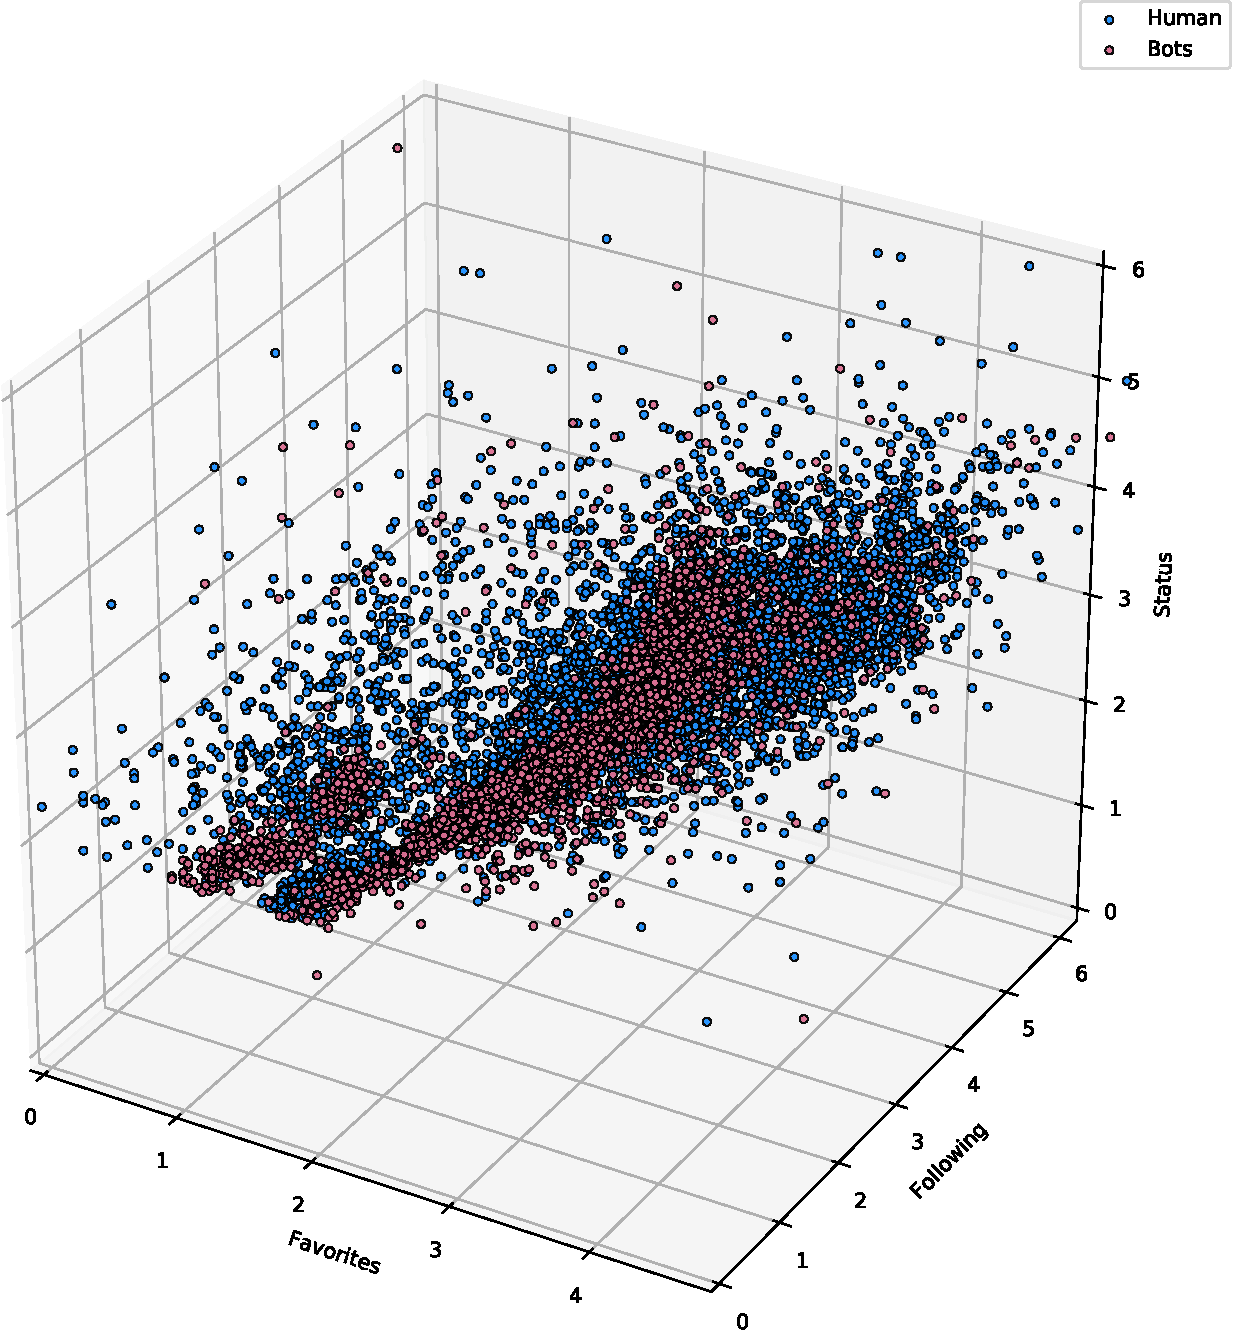
\includegraphics[width=0.6\textwidth]{FIG/3dvis_base-crop.pdf}
    \caption{We can clearly see the different distributions of humans (blue) and bots (red). All axes are plotted in log scale.}
    \label{fig:3dvis}
\end{figure}

Lastly, we would like to note the fact that \textsc{Cresci-2018} may not have been the ideal dataset and we believe that this method could work much better on higher quality data and particularly well for data with bots who deviate stronger from the norm in terms of social structure in the graph. This dataset was collected from so called ``stock Twitter'', a subset of Twitter users that mainly talk about stocks and market movements, and the data was focused on bots that aim to influence the market by shaping the perception of public opinion on Twitter through retweeting (i.e. sharing with their followers) of suspicious ``peak tweets''~\cite{cresci2018fake}. We have noticed that this is also reflected in the users contained in the datasets and that these users may not be easily and reliably identified using only profile, and graph neighborhood data. Additionally, many users in the dataset that are labelled as bots do not immediately strike us as bots upon manual review which brings the quality of the dataset into question. In general the in- and out-degrees of users in the dataset (for both human and bot accounts) seem much higher than we would expect from a random sample of Twitter users. Despite these circumstances we find that our approach works and is able to improve upon baseline classification models for ``free": it does not require any additional labelled data and simply augments existing labelled data by use of data from neighbors in the social graph. 

% Final report

\section{Conclusion}
    \label{sec:conclusion}
    In this section we will come to a conclusion.

\noindent We have collected a novel dataset of 4.6 million Twitter user profiles based on the users followed by or following users in the \textsc{Cresci-2018} dataset. In our analysis we have found a number of graph features and aggregate features that can help in bot classification. We propose a novel method to bot classification which utilizes neighborhood-based features for classification. Our method performs better than the competitors on the \textsc{Cresci-2018} dataset.

\bibliography{BIB/other}
\bibliographystyle{plain}

\newpage
\appendix
\section{Appendix}
\subsection{Labor Division}

During our work we will perform the following tasks
\bit
\item Find a fitting dataset to test our approach, est. $\sim$3h [Bebensee]
\item Scrape the social graph of accounts containted in the dataset and clean the data, est. $\sim$5h [Bebensee]
\item Read more to our approach related work, est. $\sim$2h [Nazarov]
\item Explore the graph data to find possible discrepancies between subgraphs of bots and subgraphs of real users, est. $\sim$6h [Nazarov]
\item Run experiments on the data, est. $\sim$12h [Bebensee, Nazarov]
\item Develop a classification approach based on our findings, est. $\sim$8h [Bebensee, Nazarov]
\item Evaluate our approach in experiments, determine precision, recall, AUC (area under ROC), est. $\sim$10h [Bebensee, Nazarov]
\eit

\subsection{Full disclosure with regards to dissertations/projects}

\paragraph{Bebensee:}
His research and thesis is not related to this project in any way. He is working on neural machine translation and visual question answering.

\paragraph{Nazarov:}
His research and thesis is not related to this project in any way. He is working on designing an open framework for designing, implementing, and evaluating hardware and software components for solid-state drives. 

\section{Proposal paper}

\newpage
\pagenumbering{roman}
\tableofcontents


\end{document}
